\icode{E-MM-MU-L3-261013-001}
如图所示，不可伸长的轻质细线跨过轻质滑轮连接两个质量分别为\(2m\)、\(m\)的物体\(A\)、\(B\)，质量为\(m\)的物体\(C\)中间有孔，套在细线上且可以沿细线无摩擦滑动。初始时使三个物体均处于静止状态，此时\(A\)、\(B\)离地面的高度为均为\(h\)，物体\(C\)在\(B\)上方\(h\)处。同时由静止释放三个物体，一段时间后，\(C\)与\(B\)发生碰撞并立即粘在一起。已知重力加速度大小为\(g\)，整个过程中细线末断裂，物体均可视为质点，不计阻力的影响。下列说法正确的是\paren[]

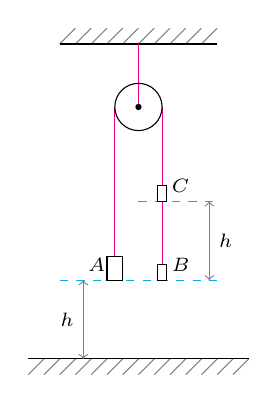
\begin{tikzpicture}[font=\scriptsize]
	\foreach \x in {1,.8,...,-.8}
		\draw[gray] (\x,.2)--++(-.2,-.2);
    \draw[thick] (-1,0)--(1,0);
	\draw[magenta] (0,0)--(0,-.8) (-.3,-.8)--(-.3,-3) (.3,-.8)--(.3,-3);
	\draw (0,-.8) circle(.3);
    \fill (0,-.8) circle(.04);
	\draw[dashed,cyan] (-1,-3)--(1,-3) (0,-2)--(1,-2);
	\draw[fill=white] (-.4,-3) rectangle(-.2,-2.7) (.36,-3) rectangle(.24,-2.8) (.36,-2) rectangle(.24,-1.8);
	\foreach \x in {-1.4,-1.2,...,1.2}
		\draw[gray] (\x,-4.2)--++(.2,.2);
	\draw (-1.4,-4)--(1.4,-4);
	\draw[<->,gray] (-.7,-3)--node[left,black]{\(h\)}(-.7,-4);
	\draw[<->,gray] (.9,-3)--node[right,black]{\(h\)}(.9,-2);
	\node at(-.3,-2.8)[left]{\(A\)};
	\node at(.3,-2.8)[right]{\(B\)};
	\node at(.3,-1.8)[right]{\(C\)};
\end{tikzpicture}
\begin{choices}
	\item 从释放三个物体到\(C\)与\(B\)发生碰撞经历的时间为\(\sqrt{\frac{h}{g}}\)
	\item 碰撞结束后\(A\)的速度为零
	\item\(A\)最终离地面的高度为\(\frac{1}{4}h\)
	\item 碰撞过程中，三个物体损失的机械能为\(mgh\)
\end{choices}
\begin{answer}
   BD\qquad 提示：\(C\) 与\(B\)碰撞是完全非弹性碰撞，绳子绷紧\(BC\)整体与\(A\)共速，又是完全非弹性碰撞
\end{answer}